

\documentclass[handout,t]{beamer}
\usepackage{graphicx,url}
\usepackage[french]{babel}   
\usepackage[utf8]{inputenc}
\usepackage{nicefrac}
\usepackage{listings}
\usepackage{lmodern}
\usepackage[T1]{fontenc}
\usepackage{shadow,palatino,wasysym}


\usepackage{amscd,array}
\usepackage{listings}
\usepackage{wrapfig}
\usepackage{lipsum}
\usepackage{galois}
\usepackage{epsfig,tabularx}


\usepackage{amsmath,pifont,amssymb,enumerate,mathtools,epsfig,bbm,calc,color,ifthen,capt-of}
%\usetheme{Berlin}
%\usecolortheme{senac}

\definecolor{senac-laranja}{rgb}{0.78,0.16,0.22}
\definecolor{senac-azul}{rgb}{0.4,.4,0.4}
\definecolor{blue}{rgb}{0.3,0.3,0.5}
\definecolor{red}{rgb}{0.78,0.16,0.22}
\definecolor{green}{rgb}{0.1,0.6,0.2}
\definecolor{orange}{rgb}{0.2,0.6,0.2}

\usetheme{CambridgeUS}
%\usecolortheme{seahorse}
\setbeamertemplate{blocks}[rounded][shadow=true]
\setbeamertemplate{items}[ball]
%\setbeamertemplate{navigation symbols}{}
\setbeamercolor{title}{bg=red!65!black, fg=white}

%\def\titre#1{\noindent \textbf{{\bf \textcolor{blue}{#1}}}\vspace{-0.2cm}\\\vspace{-0.7cm}\color{black}\rule{10cm}{.05cm}}
\def\titre#1{\noindent \textbf{{\bf \textcolor{blue}{#1}}}\\\color{black}\rule{10cm}{.05cm}}

\def\mytt#1{\texttt{\textbf{#1}}}
\def\real#1{real\{#1\}}
\def\re#1{\mathsf{R}_{#1}}
\def\mysection#1{\vspace{-1.1cm}\color{blue}
\section{#1} \vspace{-0.7cm}\color{black}\rule{10cm}{.05cm}\vspace{-0.9cm}}

\def\mysubsection#1{\vspace{-1.1cm}\color{blue}
\subsection{#1} \vspace{-0.7cm}\color{black}\rule{10cm}{.05cm}\vspace{-0.9cm}}

\def\Gamma{\sigma}
\def\Pi{\pi}

\def\preci#1{^{\mathsf{|#1|}}}
\def\fplus{\overset{\rightarrow}{\oplus}}
\def\ftimes{\overset{\rightarrow}{\otimes}}
\def\bplus{\overset{\leftarrow}{\oplus}}
\def\btimes{\overset{\leftarrow}{\otimes}}
\def\fplusi{\overset{\rightarrow}{\boxplus}}
\def\ftimesi{\overset{\rightarrow}{\boxtimes}}
\def\bplusi{\overset{\leftarrow}{\boxplus}}
\def\btimesi{\overset{\leftarrow}{\boxtimes}}

\def\ov#1{\overline{#1}}
\def\un#1{\underline{#1}}
\def\eps{\varepsilon}

\def\accf{\mathsf{acc}_F}
\def\accb{\mathsf{acc}_B}
\def\acc{\mathsf{acc}}
\def\ufp{\mathsf{ufp}}
\def\lw{\Lambda}

%\input{macros.tex}

\begin{document}

%\renewcommand{\sectionmark}[1]{\markright{\thesection\ #1}}
%\renewcommand{\subsectionmark}[1]{\markright{\thesubsection\ #1}}
%\newpagestyle{MH}
%  {}
%  {\textit{\color{blue}\rightmark} \hfill -\ \thepage\ -}
%\pagestyle{MH} 
%\frameframe{none}

\date{M. Martel, \mytt{Numl}}

                
\begin{frame}
~

\vspace{0.5cm}

%\centerline{
%{\Large \textbf{Accuracy Driven}
%}}

\medskip

\centerline{
{\Large \textbf{Strongly Typed Numerical Computations}
}}

\medskip

%\centerline{
%{\Large \textbf{ in Mixed-Precision}
%}}

\vspace{0.7cm}



\centerline{\textcolor{blue}{\sc Matthieu Martel}}

\vspace{0.7cm}

\centerline{\textcolor{blue}{\small University of Perpignan \& Numalis}}
\centerline{\textcolor{blue}{\small Laboratory of Mathematics and Physics (LAMPS)}}

\vspace{0.5cm}

\centerline{\mytt{\small mxatthieu.martel@univ-perp.fr}}

\vspace{0.8cm}


\centerline{
\begin{tabular}{cccc}

\includegraphics[width=2.2cm]{logo.png} \hspace{0.1cm}&

\includegraphics[width=1.9cm]{lamps_logo_ttt.png}\hspace{0.1cm}&

\includegraphics[width=2.3cm]{numalis.png}\hspace{0.1cm}&

\includegraphics[width=3.5cm]{onrg.jpeg}%
\end{tabular}}



\end{frame}
%%%%%%%%%%%%%%%%%%%%%%%%%%%%%%%%%%%%%%%%%%%%%%%%%%%%%%%%%%%%%%%%%%%%%%%%%
\begin{frame}
\frametitle{Introduction}


\vspace{1cm}

\textbf{Contribution:} A type system for numerical accuracy

\vspace{0.2cm}

Type inference, dependent types, ML spirit

\vspace{1cm}

\textbf{Implementation:} \mytt{Numl}

\vspace{1cm}

\textbf{Interest:} Bug elimination, early debugging, accuracy information, 

\vspace{0.2cm}

code generation with optimal precision 



\end{frame}

%%%%%%%%%%%%%%%%%%%%%%%%%%%%%%%%%%%%%%%%%%%%%%%%%%%%%%%%%%%%%%%%%%%%%%%%%
\begin{frame}
\frametitle{Summary}


\vspace{1.1cm}

~\hspace{1cm}\ding{111}\quad Introduction

\vspace{0.6cm}

~\hspace{1cm}\textcolor{red}{\ding{111}\quad An overview of \mytt{Numl}}

\vspace{0.6cm}

~\hspace{1cm}\ding{111}\quad The type system

\vspace{0.6cm}

~\hspace{1cm}\ding{111}\quad Type inference / implementation

\vspace{0.6cm}

~\hspace{1cm}\ding{111}\quad Conclusion / perspectives

\end{frame}

%%%%%%%%%%%%%%%%%%%%%%%%%%%%%%%%%%%%%%%%%%%%%%%%%%%%%%%%%%%%%%%%%%%%%%%%%
\begin{frame}
\frametitle{Types Embedding Accuracy}


%\vspace{0.1cm}

$$\color{red}
 \text{type}\    \mathtt{real\{}s,u,p\mathtt{\}}
$$

\vspace{-0.2cm}

$s$ sign of $x$, $s\in \{ +,-,0,*\}$

\vspace{0.2cm}

$u$ $\mathsf{ufp}(x)$, i.e. \textit{u}nit in the \textit{f}irst \textit{p}lace

\vspace{0.2cm}

$p$ precision (number of bits of $x$)

\vspace{0.4cm}

~\centerline{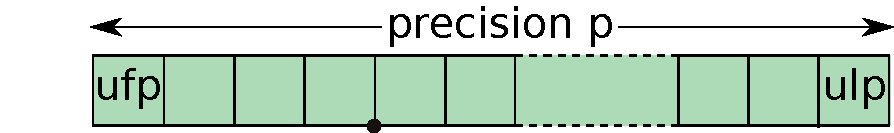
\includegraphics[width=6.5cm]{uflp.pdf}\hspace{1cm}$\color{red}err \le 2^{ulp}$}

%$$
%\mathsf{ufp}(f) = \min \big\{ i\in \mathbb{N}\ :\ 2^{i+1} > f\big\} = \lfloor \log_2(f)\rfloor
%$$



\vspace{0.4cm}

\scriptsize\color{blue}
\mytt{> 1.234 ;;}

\mytt{- : \real{+,0,53} = 1.2340000000000000 +/- 1.11022302463e-16}

\mytt{\ }

\mytt{> 1.234\{4\} ;;}

\mytt{- : \real{+,0,4} = 1.23 +/- 0.0625}
\normalsize


\end{frame}

%%%%%%%%%%%%%%%%%%%%%%%%%%%%%%%%%%%%%%%%%%%%%%%%%%%%%%%%%%%%%%%%%%%%%%%%%
\begin{frame}
\frametitle{Parameterized Types}

\scriptsize
\color{blue}

\vspace{1cm}

\mytt{> let f = fun x -> x + 1.0 ;;}

\mytt{val f : \textcolor{red}{\real{'a,'b,'c} -> \real{<expr>,<expr>,<expr>} = <fun>}}

\mytt{\ }

\mytt{> verbose true ;;}

\mytt{- : unit = ()}

\mytt{\ }

\mytt{> f ;;}


\mytt{- : \real{'a,'b,'c} -> real(((max 'b 0) +\_ (sigma+ 'a 1)),}

~\hspace{3.5cm}\mytt{((max 'b 0) +\_ (sigma+ 'a 1)),}

~\hspace{3.5cm}\mytt{((((max 'b 0) +\_ 1) -\_ (max ('b -\_ 'c) - 53))}

~\hspace{3.5cm}\mytt{-\_ (iota ('b -\_ 'c) - 53))) = <fun>}

\vspace{0.6cm}

\normalsize\color{black}
\mytt{+}, \mytt{-}, \mytt{*}, \mytt{/} real operators 

\vspace{0.2cm}

\mytt{+\_}, \mytt{-\_}, \mytt{*\_}, \mytt{/\_} integer operators


\end{frame}
%%%%%%%%%%%%%%%%%%%%%%%%%%%%%%%%%%%%%%%%%%%%%%%%%%%%%%%%%%%%%%%%%%%%%%%%%
\begin{frame}
\frametitle{Accuracy of the Results Explicited}

\scriptsize
\color{blue}

\vspace{0.1cm}

\mytt{> let f = fun x -> x + 1.0 ;;}

\mytt{val f : \real{'a,'b,'c} -> \real{<expr>,<expr>,<expr>} = <fun>}

\mytt{\ }


\mytt{> f 1.234 ;;}

\mytt{- : \real{+,1,53} = 2.2340000000000000 \textcolor{red}{+/- 2.22044604925e-16}}

\mytt{\ }

\mytt{> f 1.234\{4\} ;;}

\mytt{- : \real{+,1,5} = 2.23 \textcolor{red}{+/- 0.0625}}

\mytt{\ }

\mytt{\ }


\mytt{> (1.0e15 + 1.0) - 1.0e15 ;;}

\mytt{- : \real{+,50,54} = 1.0 \textcolor{red}{+/- 0.0625}}

\mytt{\ }

\mytt{> (1.0e16 + 1.0) - 1.0e16 ;;}

\mytt{\textcolor{red}{Error: The computed value has no significant digit. Its ufp is 0 but the ulp of the certified
value is 1}}

\vspace{0.3cm}

~\hfill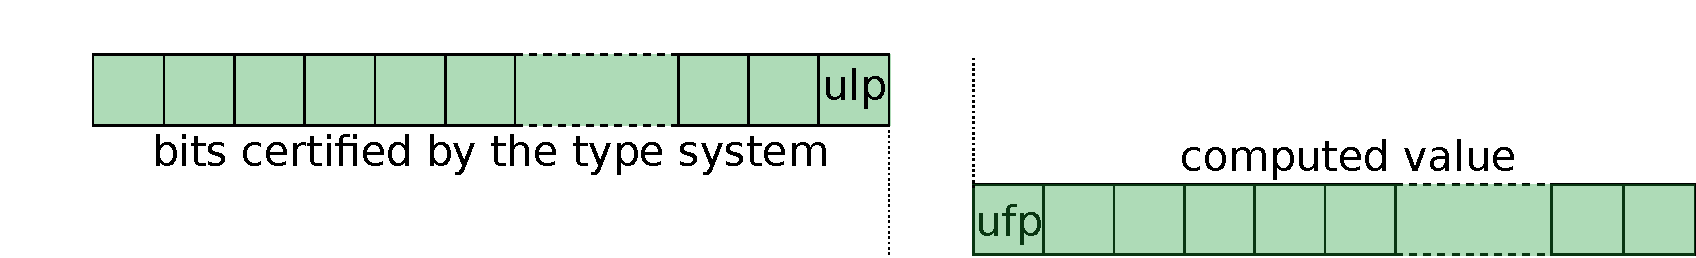
\includegraphics[width=10cm]{cancel.pdf}

\end{frame}

%%%%%%%%%%%%%%%%%%%%%%%%%%%%%%%%%%%%%%%%%%%%%%%%%%%%%%%%%%%%%%%%%%%%%%%%%
\begin{frame}
\frametitle{Recursivity and Subtyping}


$$\small
\mytt{<}\ :\ \alpha\ \longrightarrow\ \alpha\ \longrightarrow\ \mytt{bool}
$$

\scriptsize
\color{blue}

\vspace{0.1cm}


\mytt{> let rec g x = if x \textcolor{green}{<} 1.0 then x else g (x * 0.07) ;;}

\mytt{\color{red}val g : \real{+,0,53} -> \real{+,0,53} = <fun>}

\mytt{\ }

\mytt{> g 1.0;;}

\mytt{\color{red}- : \real{+,0,53} =  0.070000000000000 +/- 1.11022302463e-16}

\mytt{\ }

\mytt{> g 2.0 ;;}

\mytt{\color{red}Error: This expression has type \real{+,1,53} but an expression was expected of type \real{+,0,53}}

\normalsize
\color{black}

%\vspace{0.1cm}


$$\small
\begin{array}{c}
\real{s_1,u_1,p_1} \sqsubseteq \real{s_2,u_2,p_2} 
\iff
s_1 \preceq s_2,\quad
u_1 \le u_2,\quad
p_1 \ge p_2 + u_1 - u_2
\end{array}
$$

\vspace{0.1cm}

~\hfill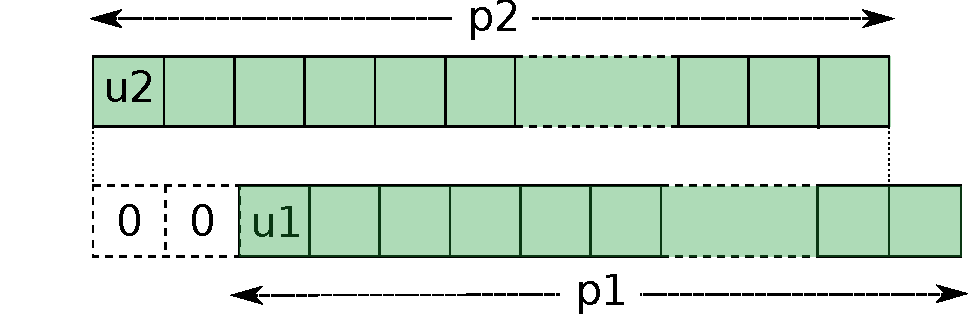
\includegraphics[width=6cm]{lttype.pdf}

\end{frame}

%%%%%%%%%%%%%%%%%%%%%%%%%%%%%%%%%%%%%%%%%%%%%%%%%%%%%%%%%%%%%%%%%%%%%%%%%
\begin{frame}
\frametitle{Monomorphic Comparisons}


\vspace{0.6cm}

$$
\mytt{<\{*,u,p\}}\ :\ \mytt{\real{*,u,p}} \longrightarrow \mytt{\real{*,u,p}} \longrightarrow 
\mytt{bool}
$$

\vspace{0.6cm}
\scriptsize
\color{blue}


\mytt{let rec g x = if x \textcolor{green}{<\{*,10,15\}} 1.0 then x else g (x * 0.07) ;;}


\mytt{\color{red}val g : \real{*,10,15} -> \real{*,10,15} = <fun>}

\mytt{\ }

\mytt{> g 2.0 ;;}

\mytt{\color{red}- : \real{*,10,15} = 0.14 +/- 0.03125}

\mytt{\ }

\mytt{> g 456.7 ;;}

\mytt{\color{red}- : \real{*,10,15} = 0.16 +/- 0.03125}

\mytt{\ }

\mytt{> g 4567.8 ;;}

\mytt{\color{red}Error: This expression has type \real{+,12,53} but an expression was expected of type \real{*,10,15}
}


\end{frame}
%%%%%%%%%%%%%%%%%%%%%%%%%%%%%%%%%%%%%%%%%%%%%%%%%%%%%%%%%%%%%%%%%%%%%%%%%
\begin{frame}
\frametitle{Another Example}

~

\vspace{0.5cm}

$$\color{green}
\frac{1}{1-x}=1+x+x^2+x^3+\ldots
$$


\vspace{0.5cm}

\scriptsize
\color{blue}

%\vspace{.2cm}


\mytt{> let rec taylor x\textcolor{green}{\{-1,25\}} xn i n =}

~ \hspace{1.55cm}\mytt{if (i>n) then 0.0\{*,10,20\} }

~ \hspace{1.55cm}\mytt{else xn + (taylor x (x*xn) (i+\_ 1) n) ;;}
 
\mytt{\color{red}val taylor : \real{*,-1,25} -> \real{*,10,20} -> int -> int -> \real{*,10,20} = <fun>
}

\mytt{\ }

\mytt{> taylor 0.2 1.0 0 5;;}

\mytt{\color{red}- : \real{*,10,20} = 1.2499 +/- 0.0009765625}

\mytt{\ }



\end{frame}

%%%%%%%%%%%%%%%%%%%%%%%%%%%%%%%%%%%%%%%%%%%%%%%%%%%%%%%%%%%%%%%%%%%%%%%%%
\begin{frame}
\frametitle{Yet Another Example}

~\hfill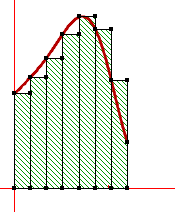
\includegraphics[width=2.5cm]{rect.png}

\vspace{-1.5cm}

\scriptsize
\color{blue}


\mytt{> let rec rectangle f a b h =}

~\hspace{0.5cm}\mytt{  if (a >= b) then }

~\hspace{1cm}\mytt{    0.0\{*,30,40\}}

~\hspace{0.5cm}\mytt{  else}

~\hspace{1cm}\mytt{    ((f a) * h) + (rectangle f (a + h) b h) ;;}

\mytt{\color{red}val rectangle : \real{<expr>,<expr>,<expr>} -> \real{+,29,41} -> \real{<expr>,<expr>,<expr>} -> \real{<expr>,<expr>,<expr>}
}

\mytt{\ }

\mytt{> let rec g x = x * x ;;}

\mytt{\color{red}val g : \real{'a,'b,'c} -> \real{<expr>,<expr>,<expr>} = <fun>}

\mytt{\ }

\mytt{> rectangle g 0.0 2.0 0.01 ;;}

\mytt{\color{red}- : \real{*,30,40} = 2.6867 +/- 0.0009765625}

\mytt{\ }

\color{black}\normalsize

\centerline{Remark: Method error not considered}

\end{frame}



%

%%%%%%%%%%%%%%%%%%%%%%%%%%%%%%%%%%%%%%%%%%%%%%%%%%%%%%%%%%%%%%%%%%%%%%%%%
\begin{frame}
\frametitle{Summary}


\vspace{1.1cm}

~\hspace{1cm}\ding{111}\quad Introduction

\vspace{0.6cm}

~\hspace{1cm}{\ding{111}\quad An overview of \mytt{Numl}}

\vspace{0.6cm}

~\hspace{1cm}\textcolor{red}{\ding{111}\quad The type system} 


\vspace{0.6cm}

~\hspace{1cm}\ding{111}\quad Type inference / implementation

\vspace{0.6cm}

~\hspace{1cm}\ding{111}\quad Conclusion / perspectives


\end{frame}


%%%%%%%%%%%%%%%%%%%%%%%%%%%%%%%%%%%%%%%%%%%%%%%%%%%%%%%%%%%%%%%%%%%%%%%%%
\begin{frame}
\frametitle{The Type System}


\vspace{1.2cm}

\color{black}
~\hspace{1cm}Dependent types

\vspace{0.8cm}

\color{red}
~\hspace{1cm}Standard typing rules

\vspace{0.8cm}

\color{black}
~\hspace{1cm}Accuracy encoded in the types of primitives


\vspace{0.8cm}

\color{red}
~\hspace{1cm}Only linear equations among integers in type expressions




\end{frame}

%%%%%%%%%%%%%%%%%%%%%%%%%%%%%%%%%%%%%%%%%%%%%%%%%%%%%%%%%%%%%%%%%%%%%%%%%
\begin{frame}
\frametitle{Terms and Types}

~

%\vspace{0.3cm}

$$
\begin{array}{rcl}
Expr\ni e&::=&\ \mathtt{x}\{s,u,p\}\in \mathbb{R}_{s,u,p}\ |\ \mathtt{i}\in \mathbb{Z}\ |\ \mathtt{b}\in \mathbb{B}
\ |\ \mathtt{id}\in\mathsf{V} \\
&&\\
&& |\  \mathtt{if}\ e_0\ \mathtt{then}\ e_1\ \mathtt{else}\ e_2
\ |\ \lambda x.e
\ |\ e_0\ e_1\ |\ t\\
&&\\
Types \ni t&::=&|\ \mathtt{int}\ |\ \mathtt{bool}\ |\ \real{e_0,e_1,e_1}\ |\ \alpha\ |\ \Pi x:e_0.e_1\ 
\end{array}
$$

\color{blue}

\vspace{0.7cm}

Note: $t_0 \rightarrow t_1 \ \equiv\ \Pi x:t_0.t_1 \quad (x\ \text{not free in}\ t_1)$

\vspace{0.5cm}


Higher order constants: \mytt{+, -, *, /, +\_, -\_, *\_, /\_}

\end{frame}

%%%%%%%%%%%%%%%%%%%%%%%%%%%%%%%%%%%%%%%%%%%%%%%%%%%%%%%%%%%%%%%%%%%%%%%%%
\begin{frame}
\frametitle{Typing Rules}

\small


$$
\frac{}
     {\Gamma \vdash \texttt{i} :\ \mathtt{int} }\quad\textsc{(Int)}
	 \hspace{2cm}
\frac{}
     {\Gamma \vdash \texttt{b } :\ \mathtt{bool} }\quad\textsc{(Bool)}
$$

$$\color{red}
     \frac{\mathsf{ufp}(\texttt{x})\le u\quad \mathsf{sign}(\texttt{x})\prec s
     }
     {\Gamma \vdash \texttt{x\{s,u,p\}}\ :\real{s,u,p} }\quad\textsc{(Real)}
\hspace{2cm}\color{black}
\frac{\mathtt{id} : t \in \Gamma}
     {\Gamma \vdash \mathtt{id}\ :\ t }\quad\textsc{(Var)}
$$

$$
\frac{
\Gamma \vdash e_0\ :\ \mathtt{bool}\hspace{1cm}\Gamma \vdash e_1\ :\ t_1\hspace{1cm} \Gamma \vdash e_2\ :\ t_2
\hspace{1cm} t=t_1\sqcup t_2}
{\Gamma\vdash \mathtt{if}\ e_0\ \mathtt{then}\ e_1\ \mathtt{else}\ e_2\ :\  t}\quad\textsc{(Cond)}
$$

$$
\frac{\Gamma,x :t_1 \vdash e :  t_2}
     {\Gamma \vdash \lambda x.e : \Pi x:t_1 .  t_2}\quad\textsc{(Abs)}
%\hspace{2cm}
$$

$$\color{red}
\frac{\Gamma \vdash e_1 : \Pi x: t_0. t_1\hspace{1cm} \Gamma \vdash e_2 :  t_2
\hspace{1cm} \textcolor{green}{t_2\sqsubseteq t_0}
}
     {\Gamma \vdash e_1\ e_2 :  t_2[x\mapsto e_2]}\quad\textsc{(App)}
$$


\end{frame}


%%%%%%%%%%%%%%%%%%%%%%%%%%%%%%%%%%%%%%%%%%%%%%%%%%%%%%%%%%%%%%%%%%%%%%%%%
\begin{frame}
  \frametitle{Type of Functional Constants}

\small
  
  $$
  \begin{array}{rcl}
\mathtt{+}~ &:& \Pi \mathtt{s_1}:\texttt{int},\mathtt{u_1}:\texttt{int}, \mathtt{p_1}:\texttt{int},\mathtt{s_2}:\texttt{int}, \mathtt{u_2}:\texttt{int}, \mathtt{p_2}:\texttt{int}.\\
&&~\quad\real{s_1,u_1,p_1}\rightarrow\real{s_2,u_2,p_2}\\
&&~\quad
\rightarrow\real{\mathcal{S}_+(\mathtt{s_1},\mathtt{s_2}),
\mathcal{U}_+(\mathtt{s_1},\mathtt{u_1},\mathtt{s_2},\mathtt{u_2}),
\mathcal{P}_+(\mathtt{u_1},\mathtt{p_1},\mathtt{u_2},\mathtt{p_2})}
\end{array}
  $$
  
\scriptsize

\vspace{0.3cm}

$$\color{red}
\begin{array}{rcl}
  \mathcal{U}_+(\mathtt{s_1},\mathtt{u_1},\mathtt{s_2},\mathtt{u_2}))&=&\max(\mathtt{u_1},\mathtt{u_2})+\sigma_+(\mathtt{u_1},\mathtt{u_2})\\
  &&\\
\mathcal{P}_+(\mathtt{u_1},\mathtt{p_1},\mathtt{u_2},\mathtt{p_2}) &=&\max(\mathtt{u_1},\mathtt{u_2})+\sigma_+(\mathtt{u_1},\mathtt{u_2})-
\max(\mathtt{u_1}-\mathtt{p_1},\mathtt{u_2}-\mathtt{p_2})-\iota(\mathtt{u_1}-\mathtt{p_1},\mathtt{u_2}-\mathtt{p_2})
\end{array}
$$


\vspace{0.1cm}

\tiny\color{blue}
$$
\begin{array}{ccc}
\mathcal{S}_+&&
\\
\begin{array}{c|c|c|c|c}
 \mathtt{s_1} \backslash \mathtt{s_2}
      &\quad 0 \quad& + & - & \quad\top\quad \\
\hline	  
\begin{array}{c}
\\ 0\\ \\
\end{array}    & 0 & + & - & \top \\
\hline
+    & + & + & 
\begin{array}{c}
+ \ \text{if}\ \mathtt{u_1}<\mathtt{u_2}\\
- \ \text{if}\ \mathtt{u_2}<\mathtt{u_1}\\
\top\ \text{otherwise}
\end{array}&\top\\
\hline
-     & - & 
\begin{array}{c}
+ \ \text{if}\ \mathtt{u_2}<\mathtt{u_1}\\
- \ \text{if}\ \mathtt{u_1}<\mathtt{u_2}\\
\top\ \text{otherwise}
\end{array}
 & - &\top\\
\hline
\begin{array}{c}
\\ \top\\ \\
\end{array} &\top &\top&\top&\top
\end{array}
&\hspace{1cm}&
\begin{array}{c}
  \iota(x,y)=\left\{
\begin{array}{l}
  1\ \text{if}\ x=y\\
  0\ \text{otherwise}
\end{array}\right.
\\
\\
\sigma_+\\
\begin{array}{c|cccc}
  & 0 & + & - & \top \\
  \hline
0& 0 & 0  & 0 & 0 \\
+& 0 & 1 & 0 & 1\\
-& 0 & 0 & 1 & 1\\
\top&0&1 & 1 &1\\
\end{array}
\end{array}
\end{array}
$$
\end{frame}


%%%%%%%%%%%%%%%%%%%%%%%%%%%%%%%%%%%%%%%%%%%%%%%%%%%%%%%%%%%%%%%%%%%%%%%%%
\begin{frame}
\frametitle{Summary}


\vspace{1.1cm}

~\hspace{1cm}\ding{111}\quad Introduction

\vspace{0.6cm}

~\hspace{1cm}{\ding{111}\quad An overview of \mytt{Numl}}

\vspace{0.6cm}

~\hspace{1cm}{\ding{111}\quad The type system} 


\vspace{0.6cm}

~\hspace{1cm}\textcolor{red}{\ding{111}\quad Type inference / implementation}

\vspace{0.6cm}

~\hspace{1cm}\ding{111}\quad Conclusion / perspectives


\end{frame}


%%%%%%%%%%%%%%%%%%%%%%%%%%%%%%%%%%%%%%%%%%%%%%%%%%%%%%%%%%%%%%%%%%%%%%%%%
\begin{frame}
\frametitle{Type Inference / Unification}


~

\vspace{0.2cm}

\color{black}
~\hspace{1cm}Type variables represented by references 

\vspace{0.8cm}

\color{red}
~\hspace{1cm}Type \mytt{real} contains references


\vspace{0.8cm}

\color{black}
~\hspace{1cm}Standard type inference and unification


\vspace{0.8cm}

\color{red}
~\hspace{1cm}Partial evaluation of types (expression simplification)

\vspace{0.8cm}

\color{black}
~\hspace{1cm}Unification of reals relies on a call to \mytt{Z3}

\end{frame}


%%%%%%%%%%%%%%%%%%%%%%%%%%%%%%%%%%%%%%%%%%%%%%%%%%%%%%%%%%%%%%%%%%%%%%%%%
\begin{frame}
\frametitle{Type Inference: Case of Application}


\vspace{0.2cm}\small

~\hspace{0.5cm}\mytt{typeCheck} $(e_1\ e_2)\ \sigma$ =

~

~\hspace{1.5cm}$t$ = \mytt{newTypeVar ()} ; $t'$ = \mytt{newTypeVar ()} ;

~

~\hspace{1.5cm}$t_1$ = \mytt{typeCheck} $e_1\ \sigma$ ; $t_2$ = \mytt{typeCheck} $e2\ \sigma$ ;

~

~\hspace{1.5cm}$t_1'$ = \mytt{simplify} $t_1$ ; $t_2'$ = \mytt{simplify} $t_2$ ;

~

~\hspace{1.5cm}$argType$ = \mytt{getArgType} $t_1'\ \sigma$ ;

~

~\hspace{1.5cm}\mytt{assert} $t_2' \ \sqsubseteq\ argType$ ; \quad \textcolor{green}{(relaxation)}

~

~\hspace{1.5cm}\mytt{unify} $t_2'\ t$ ;

~

~\hspace{1.5cm}$\alpha$ = \mytt{newVar()} ; \mytt{unify} $t_1'\ (\pi a : t.t')$ ; 

~

~\hspace{1.5cm}\mytt{return} $t'$



\end{frame}


%%%%%%%%%%%%%%%%%%%%%%%%%%%%%%%%%%%%%%%%%%%%%%%%%%%%%%%%%%%%%%%%%%%%%%%%%
\begin{frame}
\frametitle{Unification of Reals}

~

\vspace{0.3cm}

If no type variable:

~

%~\hspace{1.5cm}
\centerline{\color{blue}Maximize ufp, minimize accuracy}

\vspace{0.7cm}

\centerline{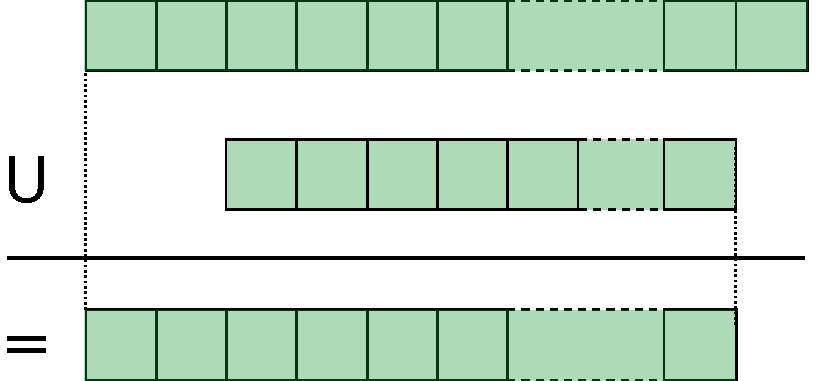
\includegraphics[width=5.5cm]{unify.pdf}}

\vspace{0.7cm}

Otherwise \mytt{solve} \ $e_{s_1} = e_{s_2}\ \wedge\ e_{u_1} = e_{u_2}\wedge\ e_{p_1} = e_{p_2}$

\end{frame}

%%%%%%%%%%%%%%%%%%%%%%%%%%%%%%%%%%%%%%%%%%%%%%%%%%%%%%%%%%%%%%%%%%%%%%%%%
\begin{frame}
\frametitle{Example of Equations Sent to \mytt{Z3}}

~


\vspace{0.5cm}


\scriptsize
\color{blue}

%


\mytt{> let rec taylor x{\{-1,25\}} xn i n =}

~ \hspace{1.55cm}\mytt{if (i>n) then 0.0\{*,10,20\} }

~ \hspace{1.55cm}\mytt{else xn + (taylor x (x*xn) (i+\_ 1) n) ;;}
 
\mytt{\color{red}val taylor : \real{*,-1,25} -> \real{*,10,20} -> int -> int -> \real{*,10,20} = <fun>
}

\vspace{.7cm}

\small\
$$\color{black}
\left\{
\begin{array}{l}
\mathcal{S}_+(\alpha, \beta, \gamma, \delta) = *\\
\\
\max( \alpha, \beta) + \sigma_+( \gamma, \delta) = 10\\
\\
 \max( \alpha,\beta ) + 1 - max (\alpha - \gamma,\beta - \delta) - \iota (\alpha -\gamma,\beta - \delta)
=20
\end{array}
\right.
$$

\end{frame}

%%%%%%%%%%%%%%%%%%%%%%%%%%%%%%%%%%%%%%%%%%%%%%%%%%%%%%%%%%%%%%%%%%%%%%%%%
\begin{frame}
  \frametitle{More Examples}


\scriptsize
\color{blue}
 \mytt{let deriv f x h = ((f (x + h)) - (f x)) / h ;;} \\
\mytt{let g x = x*x - 5.0*x + 6.0 ;;}\\
\mytt{deriv g 1.0 0.1;;}\\
~\\\color{red}
\mytt{- : \real{*,5,52} = -2.900000000000000 +/- 7.1054273576e-15}\\

\vspace{0.5cm}

\color{blue}
\mytt{let rec newton x\{10,20\} n f fprime =}\\
~\hspace{.5cm}\mytt{  if (n=0) then x}\\ 
~\hspace{.5cm}\mytt{  else let xnew = (x-((f x)/(fprime x)))}\\
~\hspace{1.55cm}\mytt{in (newton xnew (n-\_ 1) f fprime) ;;}\\
~\\ \color{red}
\mytt{\real{*,10,20} -> int -> (real{*,10,20} -> real{0,0,21})} \\
\mytt{-> (real{*,10,20} -> real{0,-9,21}) -> real{*,10,20}}\\
~\\
\color{blue}
\mytt{let g x = (x*x) - (5.0*x) + 6.0 ;;}\\
\mytt{let gprime x = 2.0 * x - 5.0 ;;}\\
\mytt{ newton 9.0 5 g gprime ;;}\\
~\\\color{red}
\mytt{- : real\{*,10,20\} = 3.0073 +/- 0.0009765625}\\


\end{frame}


%%%%%%%%%%%%%%%%%%%%%%%%%%%%%%%%%%%%%%%%%%%%%%%%%%%%%%%%%%%%%%%%%%%%%%%%%
\begin{frame}
\frametitle{Summary}


\vspace{1.1cm}

~\hspace{1cm}\ding{111}\quad Introduction

\vspace{0.6cm}

~\hspace{1cm}{\ding{111}\quad An overview of \mytt{Numl}}

\vspace{0.6cm}

~\hspace{1cm}{\ding{111}\quad The type system} 


\vspace{0.6cm}

~\hspace{1cm}{\ding{111}\quad Type inference / implementation}

\vspace{0.6cm}

~\hspace{1cm}\textcolor{red}{\ding{111}\quad Conclusion / perspectives}


\end{frame}
 %%%%%%%%%%%%%%%%%%%%%%%%%%%%%%%%%%%%%%%%%%%%%%%%%%%%%%%%%%%%%%%%%%%%%%%%
\begin{frame}
\frametitle{Conclusion / Perspectives}


~

\vspace{0.4cm}

\color{black}
~\hspace{1cm}Interpreter uses \mytt{GMP} (precision given by types)

\vspace{0.8cm}

%\color{red}
~\hspace{1cm}Compiler not yet implemented


\vspace{0.8cm}

\color{black}
~\hspace{1cm}Improve typable terms by constraint relaxation: 


\vspace{0.5cm}

\color{blue}
~\hspace{1.5cm}Improved types of primitives

\vspace{0.5cm}

%\color{black}
~\hspace{1.5cm}Modified type inference with global constraint solving

\end{frame}


%%%%%%%%%%%%%%%%%%%%%%%%%%%%%%%%%%%%%%%%%%%%%%%%%%%%%%%%%%%%%%%%%%%%%%%%%
\begin{frame}

  ~

  \vspace{0.3cm}
  
\centerline{\color{red}{\huge{ \bf ?~ \hspace{0.3cm}~\color{black} ?~ \hspace{0.3cm}~\color{red} ?~ \hspace{0.3cm}~\color{black} ?~ \hspace{0.3cm}~\color{red} ?~ \hspace{0.3cm}~\color{black} ?~ \hspace{0.3cm}~\color{red} ?~ \hspace{0.3cm}~\color{black} ?
  }}}

  \vspace{1cm}

\centerline{\color{black}{\huge{ \bf ?~~ \hspace{0.3cm}~\color{red} ? \hspace{0.3cm}~\color{black} ?~ \hspace{0.3cm}~\color{red} ?~ \hspace{0.3cm}~\color{black} ?~ \hspace{0.3cm}~\color{red} ?~ \hspace{0.3cm}~\color{black} ?~ \hspace{0.3cm}~\color{red} ?
}}}

\vspace{1cm}

\centerline{\color{red}{\huge{ \bf ?~ \hspace{0.3cm}~\color{black} ?~ \hspace{0.6cm}~\color{blue} QUESTIONS~ \hspace{0.6cm}~\color{red} ?~ \hspace{0.3cm}~\color{black} ?
  }}}

  \vspace{1cm}

\centerline{\color{black}{\huge{ \bf ?~~ \hspace{0.3cm}~\color{red} ? \hspace{0.3cm}~\color{black} ?~ \hspace{0.3cm}~\color{red} ?~ \hspace{0.3cm}~\color{black} ?~ \hspace{0.3cm}~\color{red} ?~ \hspace{0.3cm}~\color{black} ?~ \hspace{0.3cm}~\color{red} ?
}}}

  \vspace{1cm}

\centerline{\color{red}{\huge{ \bf ?~ \hspace{0.3cm}~\color{black} ?~ \hspace{0.3cm}~\color{red} ?~ \hspace{0.3cm}~\color{black} ?~ \hspace{0.3cm}~\color{red} ?~ \hspace{0.3cm}~\color{black} ?~ \hspace{0.3cm}~\color{red} ?~ \hspace{0.3cm}~\color{black} ?
  }}}

  
\end{frame}


\end{document}

















%%%%%%%%%%%%%%%%%%%%%%%%%%%%%%%%%%%%%%%%%%%%%%%%%%%%%%%%%%%%%%%%%%%%%%%%%
\begin{frame}
\frametitle{Another Example}


~\hfill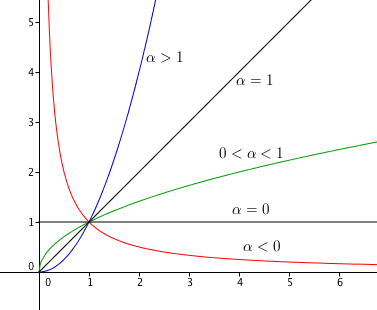
\includegraphics[width=3.5cm]{pow.png}

\vspace{0.2cm}

\scriptsize
\color{blue}

\mytt{> let rec pow x n = if (n=0) then 1.0 else x * (pow x (n -\_ 1)) ;;}
 
\mytt{\color{red}val pow : \real{+,-1,54} -> int -> \real{+,0,53} = <fun>}

\mytt{\ }

\mytt{> let rec pow x n = if (n=0) then 1.0\{5,24\} else x*(pow x (n-\_ 1)) ;; }

\mytt{\color{red}val pow : \real{+,4,25} -> int -> \real{+,5,24} = <fun>}

\mytt{\ }

\mytt{> pow 3.0 2 ;;}

\mytt{\color{red}- : \real{+,5,24} = 9.000000 +/- 1.90734863281e-06}

\mytt{\ }

\mytt{> pow 3.0 4 ;;}

\mytt{\color{red}Error: The computed value is out of the range of the certified values. Its ufp is 6 which is greater than the ufp 5 in the type of the result
}


\end{frame}



%%%%%%%%%%%%%%%%%%%%%%%%%%%%%%%%%%%%%%%%%%%%%%%%%%%%%%%%%%%%%%%%%%%%%%%%%
\begin{frame}
\frametitle{Run-Time Range Check}

\vspace{0.6cm}

\scriptsize
\color{blue}

\mytt{> let rec sum l=if (l=[]) then 0.0 else (hd l)+(sum (tl l)) ;;}

\mytt{\color{red}val f : \real{0,0,53} list -> \real{0,0,53} = <fun>}

\mytt{\ }


\mytt{> let rec sum l=if (l=[]) then 0.0\{*,10,20\} else (hd l)+(sum (tl l)) ;;}

\mytt{\color{red}val sum : \real{*,10,20} list -> \real{*,10,20} = <fun>}

\mytt{\ }

\mytt{> sum [1.1;2.2;3.3] ;;}

\mytt{\color{red}- : \real{*,10,20} = 6.6000 +/- 0.0009765625}

\mytt{\ }

\mytt{> sum [1111.1;2222.2;3333.3] ;;}

\mytt{\color{green}Error: The computed value is out of the range of the certified values. Its ufp is 12 which is greater than the ufp 10 in the type of the result}

\vspace{0.4cm}

~\hfill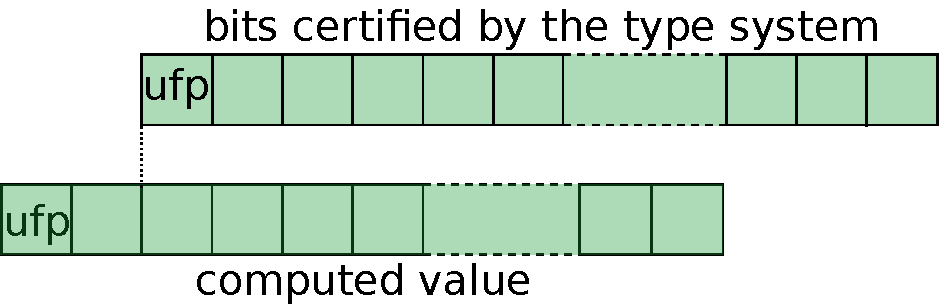
\includegraphics[width=6cm]{overflow.pdf}

\end{frame}
